\chapter{Correlating Different Devices}

\todo{describe how different devices can be correlated}

\section{Triggered Devices}

\todo{if event has no time information, event definition is the trigger}

\section{Triggerless Devices}

\todo{event needs to be defined by the metronome}

\section{Mixing Devices}

\todo{set triggered device first, start/stop information from frame is taken as event (metronome information replacement) and subsequent untriggered devices use this time window to define the event}


\begin{figure}[h]
	\centering
	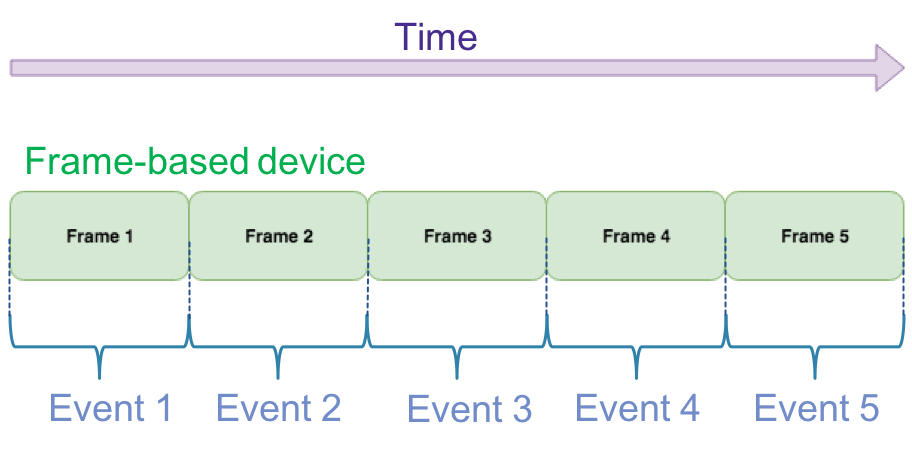
\includegraphics[width=0.66\textwidth]{framebaseddevice.png}
	\caption{text here}
	\label{fig:framebased}
\end{figure}


\begin{figure}[h]
        \centering
        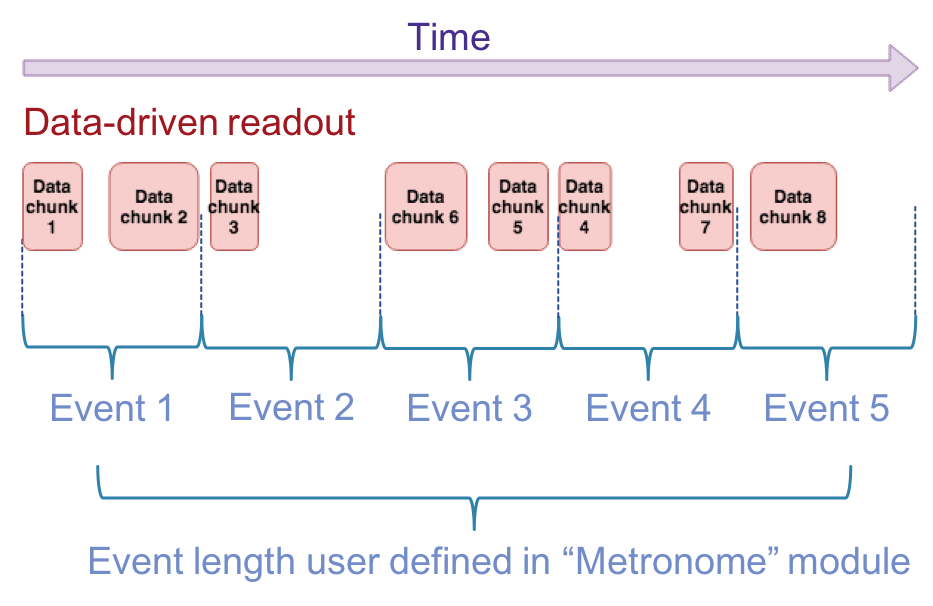
\includegraphics[width=0.66\textwidth]{datadrivendevice.png} 
        \caption{text here}
        \label{fig:datadriven}
\end{figure}



\begin{figure}[h]
        \centering
        \includegraphics[width=0.66\textwidth]{datadrivenandframebaseddevice.png} 
        \caption{text here}
        \label{fig:datadrivenandframebased}
\end{figure}


